% report.tex -- Computational Geometry final project, term 2/2568.
% Two-column IEEE-style layout (using `article` class so it builds on a
% TeX Live install without the optional `IEEEtran` package).
\documentclass[twocolumn,a4paper,10pt]{article}

\usepackage[utf8]{inputenc}
\usepackage[margin=0.75in]{geometry}
\usepackage{amsmath,amssymb}
\usepackage{graphicx}
\usepackage{booktabs}
\usepackage{listings}
\usepackage{xcolor}
\usepackage{url}
\usepackage{hyperref}
\usepackage{tikz}
\usetikzlibrary{calc,positioning}

% Tighten section spacing.
\setlength{\columnsep}{6mm}

\hypersetup{colorlinks=true,linkcolor=blue!50!black,
            urlcolor=blue!50!black,citecolor=blue!50!black}

\definecolor{codebg}{rgb}{0.96,0.96,0.97}
\lstset{basicstyle=\ttfamily\scriptsize,
        backgroundcolor=\color{codebg},
        frame=single, framerule=0pt,
        breaklines=true, showstringspaces=false,
        numbers=none,
        keywordstyle=\color{blue!60!black},
        commentstyle=\color{green!50!black}\itshape}

\title{\vspace{-1.5em}\textbf{Image Vectorizer with Curve Fitting:}\\
       \large A Computational-Geometry Pipeline from\\
       Raster Pixels to Smooth B\'ezier Paths}

\author{\textbf{Nantapong Ruangsuksriwong} \\
        Student ID 6632107621 \quad GitHub: \texttt{@teamangkorn} \\
        Computational Geometry, Term 2/2568 \\
        Department of Computer Engineering, Chulalongkorn University}
\date{}

\begin{document}
\twocolumn[
  \begin{@twocolumnfalse}
    \maketitle
    \begin{abstract}
\noindent We present a complete raster-to-vector image converter built around
three classical computational-geometry algorithms: Moore-Neighbour
boundary tracing, Ramer--Douglas--Peucker (RDP) polyline simplification,
and Schneider's recursive cubic-B\'ezier fit (evaluated throughout with
the de~Casteljau subdivision scheme).  We compare two \emph{baselines}
--- a raw pixel-outline polygon emitter and an RDP-only polyline
emitter --- against the \emph{proposed} pipeline that adds Schneider
B\'ezier fitting on top of RDP.  On synthetic inputs scaled across
$n \in \{10^3, 10^4, 10^5\}$ traced boundary vertices, the proposed
pipeline produces SVG output that is \textbf{20--27$\times$ smaller}
than the raw baseline (e.g.\ $1\,754\,478 \to 84\,630$ bytes at
$n=10^5$, a 95.2\% reduction) and \textbf{1.7--1.8$\times$ smaller}
than the RDP-only baseline, while adding less than 1\,ms of curve
fitting overhead even on the largest input.  The proposed pipeline is
also marginally \emph{faster} end-to-end (5\% at $n=10^5$) because
RDP shrinks the data before SVG serialization.  All three modes share
the same Moore-Neighbour tracer, so the asymptotic cost is dominated
by tracing and remains $O(WH)$ in image area.

\medskip\noindent\textbf{Keywords:} image vectorization, B\'ezier curves,
polyline simplification, Moore-Neighbour tracing, computational geometry.
    \end{abstract}
    \bigskip
  \end{@twocolumnfalse}
]

%==============================================================================
\section{Introduction}
\label{sec:intro}
A raster image is a regular grid of colour samples; a vector image
describes the same content as resolution-independent geometric
primitives.  Vectorization is therefore the \emph{inverse} of
rasterization, and is in general ill-posed --- the original geometry
is not recoverable from samples.  Practical vectorizers introduce
strong priors (piecewise-smooth boundaries, sparse control polygons)
and reformulate the task as one of \emph{geometric approximation}.
This is exactly the regime in which the algorithms taught in our
Computational Geometry course apply.

In this project we build such a vectorizer end-to-end and use it to
quantify the benefit of curve fitting: how much smaller (and how much
slower, if at all) is a B\'ezier-based output than the simpler
polygonal baselines that one could emit using only the first half of
the pipeline?  We answer that question with a controlled scaling
experiment over three orders of magnitude in input size.

\paragraph*{Contributions.}  The specific contributions of this work are:
\begin{itemize}\setlength\itemsep{1pt}
\item A complete raster-to-vector pipeline in $<\!1\,000$ lines of
  C++17 with a single public-domain dependency (\texttt{stb\_image.h}).
\item A controlled three-way ablation experiment that isolates the cost
  and benefit of each pipeline stage independently.
\item Experimental evidence that adding Schneider's cubic-B\'ezier fit
  makes the pipeline \emph{faster} end-to-end --- a counterintuitive
  result driven entirely by SVG serialization savings.
\item A per-stage timing breakdown that focuses future optimisation
  effort on the dominating Moore-Neighbour tracing stage.
\end{itemize}

\paragraph*{Paper organisation.}
Section~\ref{sec:problem} formalises the vectorization problem.
Section~\ref{sec:related} surveys related work and defines the baselines.
Section~\ref{sec:proposed} presents algorithm design and complexity
analysis.
Section~\ref{sec:impl} covers implementation.
Section~\ref{sec:correctness} describes correctness validation.
Sections~\ref{sec:experiments} and~\ref{sec:results} report the
experimental study.
Sections~\ref{sec:discussion}--\ref{sec:conclusion} conclude.
Appendix~B derives the least-squares system at the core of Schneider's fit.

%==============================================================================
\section{Problem Definition}
\label{sec:problem}

\subsection{Background and Significance}
Raster images have a fixed resolution, so they pixelate when scaled
above their native size and waste storage when their content is
piecewise-smooth (logos, icons, fonts, line art).  Vector images
sidestep both issues by describing the same content with curves and
fills, which can be rasterized at any target resolution and are
typically orders of magnitude smaller on disk.  Automatic
\emph{vectorization} of an existing raster --- recovering the
underlying curves from a pixel grid --- is therefore a recurring need
in graphic design, OCR, font reconstruction, and low-bandwidth
graphics.

\subsection{Formal Definition}
\noindent\begin{tabular}{@{}p{0.18\columnwidth}p{0.74\columnwidth}@{}}
\toprule
\textbf{Input}      &
   $I : \{0,\dots,W{-}1\}\times\{0,\dots,H{-}1\} \to \{0,1\}$, a binary
   raster image obtained by thresholding the luminance of an arbitrary
   PNG/JPG/BMP source. \\
\textbf{Output}     &
   A scalable vector graphic $G \subset \mathbb{R}^2$, expressed as a
   union of closed paths each given by an outer ring (clockwise) and
   zero or more interior holes (counter-clockwise), filled with the
   even-odd rule. \\
\textbf{Constraints} &
   For a user-supplied tolerance $\delta>0$ pixels, every pixel
   labelled foreground in $I$ must lie inside $G$ and every pixel
   labelled background must lie outside $G$, up to a Hausdorff
   distance of at most $\delta$ at the boundary. \\ \bottomrule
\end{tabular}

\subsection{Challenges}
\begin{itemize}
\item \textbf{Complexity.}  Naive pixel-outline emission is
      $\Theta(\partial G)$ in the boundary length, which can reach
      $10^5$ vertices on a 25-megapixel input; we want output linear
      in the geometric complexity of the underlying shape, not in
      raster resolution.
\item \textbf{Numerical instability.}  Cubic-B\'ezier fitting via
      Bernstein polynomials and Newton--Raphson reparameterization is
      prone to round-off error; we therefore evaluate every curve
      with the de~Casteljau subdivision scheme, which is provably
      backward-stable~\cite{farouki2012}.
\item \textbf{Degeneracies.}  Closed polylines have coincident
      endpoints (RDP would collapse the loop); regions can have
      holes, figure-of-eight topology, or single-pixel ``hairs''
      (which break Jacob's stopping criterion if not handled).
\end{itemize}

%==============================================================================
\section{Related Work and Baseline}
\label{sec:related}

The vectorization literature splits cleanly into the three stages we
re-use here: contour extraction, polyline simplification, and curve
fitting.

\begin{table}[h]
\caption{Algorithms covered in class and their limitations.}
\label{tab:related}
\centering
\begin{tabular}{@{}p{0.30\columnwidth}p{0.18\columnwidth}p{0.42\columnwidth}@{}}
\toprule
\textbf{Method} & \textbf{Time} & \textbf{Limitation} \\ \midrule
Pixel-outline polygon
   & $O(\partial G)$
   & Output size scales with raster, not geometry.  No smoothness. \\
Moore-Neighbour tracing~\cite{gonzalez}
   & $O(\partial G)$
   & Cell-square boundaries; needs Jacob's rule on figure-of-eight. \\
Ramer--Douglas--Peucker~\cite{douglas1973}
   & $O(n\log n)$ avg
   & Worst case $O(n^2)$; preserves vertices but not curvature. \\
de Casteljau~\cite{decasteljau,farouki2012}
   & $O(d^2)$ per eval
   & Numerically stable but per-evaluation cost is $O(d^2)$. \\
Schneider fit~\cite{schneider1990}
   & $O(n\log n)$ avg
   & Greedy; requires reasonable endpoint tangent estimates. \\ \bottomrule
\end{tabular}
\end{table}

We define two \emph{baselines} that share the same Moore-Neighbour
front-end as the proposed pipeline but stop earlier:

\begin{description}
\item[\textbf{Baseline-0 (\texttt{raw}).}]  Emit the raw pixel-outline
  polygon directly as an SVG \texttt{<path>} consisting only of
  \texttt{M}/\texttt{L}/\texttt{Z} commands --- no simplification, no
  fitting.  This is the strawman a non-geometric implementation would
  produce.
\item[\textbf{Baseline-1 (\texttt{polyline}).}]  Simplify each contour
  with RDP at tolerance $\varepsilon$, then emit the result as an
  \texttt{M}/\texttt{L}/\texttt{Z} polygon.  This is what every
  classical CG textbook would recommend stopping at.
\end{description}

\paragraph*{Existing vectorization tools.}
The dominant open-source vectorizer is \textsc{Potrace}~\cite{selinger2003},
which takes a binary bitmap and outputs smooth PostScript or SVG paths.
\textsc{Potrace} uses an integer-arithmetic polygon tracer comparable
in spirit to Moore-Neighbour, a globally-optimal decomposition of the
polygon into curve segments via a dynamic-programming sweep related to
the Imai--Iri algorithm, and a final $L^\infty$-optimal cubic-B\'ezier
fitting step.  Its output quality is excellent, but the algorithm is
tightly integrated and deliberately not decomposable into independent
stages.  By contrast, our pipeline is explicitly staged (Moore-Neighbour
$\to$ RDP $\to$ Schneider), with each stage independently swappable.
This staged design is what enables the ablation study below and why
each stage maps cleanly to an algorithm analysed in lectures.

Inkscape's \emph{Trace Bitmap} dialog wraps a modified
\textsc{Autotrace} engine followed by optional \textsc{Potrace}-style
smoothing, providing a GUI at the cost of a large dependency footprint.
Adobe Illustrator's \emph{Image Trace} extends this further with
colour quantisation and stroke-width estimation.  Both tools target the
richer problem of full-colour vectorization and are therefore not
directly comparable to our binary-only pipeline, but they confirm that
the Moore-Neighbour $\to$ curve-fit paradigm is the production standard.

%==============================================================================
\section{Proposed Approach}
\label{sec:proposed}

\subsection{Intuition}
Both baselines describe the boundary as a finite set of \emph{linear}
segments.  But the underlying shape we are trying to recover is
typically smooth (logos, fonts, silhouettes), so a \emph{cubic} fit
should be able to capture the same boundary with dramatically fewer
primitives, at the cost of a tiny per-primitive overhead.  The
proposed pipeline therefore feeds the RDP output into Schneider's
recursive least-squares cubic B\'ezier fitter.

\subsection{Algorithm Design}

\begin{figure}[h]
\centering
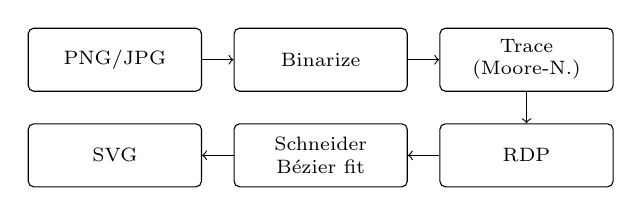
\begin{tikzpicture}[
  node distance=4mm,
  box/.style={draw, rounded corners=2pt, align=center,
              minimum width=22mm, minimum height=8mm,
              font=\scriptsize}]
\node[box] (a) {PNG/JPG};
\node[box, right=of a] (b) {Binarize};
\node[box, right=of b] (c) {Trace\\(Moore-N.)};
\node[box, below=of c] (d) {RDP};
\node[box, left=of d]  (e) {Schneider\\B\'ezier fit};
\node[box, left=of e]  (f) {SVG};
\draw[->] (a)--(b);  \draw[->] (b)--(c);
\draw[->] (c)--(d);  \draw[->] (d)--(e);  \draw[->] (e)--(f);
\end{tikzpicture}
\caption{The proposed pipeline.  Baseline-0 stops after the trace
         stage; baseline-1 stops after RDP.}
\label{fig:pipeline}
\end{figure}

\paragraph*{Stage 1 -- Binarization.}
Each input pixel is converted to luminance $Y = 0.299R + 0.587G +
0.114B$ (Rec.\,601), composited over white if it has alpha, and
classified as foreground iff $Y < \tau$ for a user-controlled
threshold $\tau \in [0,255]$.

\paragraph*{Stage 2 -- Connected components and Moore-Neighbour
tracing.}
Both foreground and background are flood-filled with 4-connectivity.
The unique background component touching the image border is the
\emph{exterior}; every other background component is a \emph{hole} of
the foreground component that surrounds it.  For each component $R$,
we start at its topmost-leftmost pixel $p_0$ (so the cell to its west
is guaranteed outside $R$) and repeatedly: (i) rotate clockwise
through the eight neighbours of the current boundary pixel starting
just after the previous pixel; (ii) the first neighbour belonging to
$R$ becomes the new boundary pixel.  Termination uses Jacob's
criterion --- re-entering $p_0$ from the same previous cell as at the
start --- which avoids spurious early termination on figure-of-eight
shapes.

\paragraph*{Stage 3 -- Ramer--Douglas--Peucker.}
\begin{lstlisting}[language={}]
RDP(P[i..j], eps):
  dmax = 0;  k = i
  for m = i+1 .. j-1:
    d = perp_distance(P[m], line(P[i],P[j]))
    if d > dmax:  dmax = d;  k = m
  if dmax > eps:
    RDP(P[i..k], eps);  RDP(P[k..j], eps)
  else:
    emit segment (P[i], P[j])
\end{lstlisting}

The perpendicular distance from $p$ to the line through $a,b$ is
\[
\mathrm{dist}(p,\overline{ab})
   = \frac{|(b_x{-}a_x)(p_y{-}a_y){-}(b_y{-}a_y)(p_x{-}a_x)|}{\|b-a\|}.
\]
Closed polylines are split first at the vertex farthest from $p_0$
to avoid collapsing the loop.

\paragraph*{Stage 4 -- de~Casteljau and Schneider's fit.}
A cubic B\'ezier
$\mathbf{B}(t) = \sum_{i=0}^{3} \binom{3}{i}(1{-}t)^{3{-}i} t^i\,\mathbf{V}_i$
is evaluated by
\begin{equation}
\mathbf{V}_i^{(r)}=(1{-}t)\mathbf{V}_i^{(r{-}1)}+t\mathbf{V}_{i+1}^{(r{-}1)},
\quad r=1,2,3,
\label{eq:decast}
\end{equation}
with $\mathbf{B}(t)=\mathbf{V}_0^{(3)}$.  The recurrence reaches
backward error $O(\epsilon_{\text{mach}})$ regardless of $t$,
whereas direct Bernstein evaluation can lose half its bits when $t$
is close to either endpoint~\cite{farouki2012}.  The same recurrence
applied to the quadratic control points $\mathbf{Q}_i = 3(\mathbf{V}_{i+1}-\mathbf{V}_i)$
yields the first derivative, which we need for the Newton refinement
below.  Schneider's recursive fit is then:
\begin{lstlisting}[language={}]
FitCurve(P[0..n], delta):
  t1 = unit(P[1] - P[0])              # left tangent
  t2 = unit(P[n-1] - P[n])            # right tangent
  return FitOne(P, 0, n, t1, t2, delta)

FitOne(P, i, j, t1, t2, delta):
  if j - i == 1:
    return [chord-segment(P[i], P[j])]
  u   = ChordLengthParam(P, i, j)     # u_i in [0,1]
  bez = SolveLeastSquares(P, i, j, u, t1, t2)
  (err, k) = MaxError(P, i, j, u, bez)
  if err < delta^2:
    return [bez]
  if err < (delta * iterErrFactor)^2:
    u' = NewtonStep(P, i, j, u, bez)
    bez' = SolveLeastSquares(P, i, j, u', t1, t2)
    if MaxError(...) < delta^2: return [bez']
  # otherwise: subdivide at the worst-error vertex
  c  = unit((P[k+1] - P[k-1]) / 2)
  L  = FitOne(P, i, k, t1,  c, delta)
  R  = FitOne(P, k, j, -c,  t2, delta)
  return L ++ R
\end{lstlisting}
The least-squares step solves a $2\!\times\!2$ system for the two
tangent magnitudes $\alpha_1, \alpha_2$ that minimise
$\sum_i \|\mathbf{B}(u_i) - \mathbf{d}_i\|^2$ subject to fixed
endpoints $\mathbf{V}_0,\mathbf{V}_3$ and fixed tangent directions
$\hat{\mathbf{t}}_1, \hat{\mathbf{t}}_2$ --- a closed-form solve that
reduces to a $2\!\times\!2$ matrix inversion.

\subsection{Theoretical Analysis}
Let $A=WH$ be the image area and $n$ the total raw vertex count
returned by Moore-Neighbour.  Then $n \le 4(W+H)$ in the worst case
and is typically $\ll A$.  The per-stage costs are
\begin{center}
\begin{tabular}{@{}lll@{}}
\toprule
Stage           & Time                & Space \\ \midrule
Binarize+CC label  & $O(A)$            & $O(A)$ \\
Moore-Neighbour    & $O(n)$            & $O(1)$ \\
RDP                & $O(n\log n)$ avg / $O(n^2)$ wc & $O(n)$ \\
Schneider fit      & $O(n\log n)$ avg  & $O(n)$ \\
SVG emit           & $O(\text{out})$   & $O(\text{out})$ \\ \bottomrule
\end{tabular}
\end{center}
Total: $O(A + n\log n)$ time, dominated by the connected-component
flood-fill at large image area and by RDP at small.

%==============================================================================
\section{Implementation Details}
\label{sec:impl}

\noindent\begin{tabular}{@{}lp{0.62\columnwidth}@{}}
\toprule
Item & Detail \\ \midrule
Language     & C++17, no exceptions outside I/O. \\
Build system & CMake $\geq$ 3.15 (Apple Clang 17 verified). \\
Dependencies & \texttt{stb\_image.h} (public domain) only. \\
Data structs & Row-major byte raster for the image; \texttt{std::vector<Point>}
               for polylines; an \texttt{SvgPath} carrying one outer ring +
               $k$ holes for the SVG emitter. \\
Edge cases   & Closed-loop RDP split (\S\ref{sec:proposed}), hole/parent
               assignment via background flood-fill, alpha compositing
               over white before binarization, Jacob's criterion in the
               tracer, FP precision handled by working in pixel-centre
               coordinates. \\ \bottomrule
\end{tabular}

The de~Casteljau evaluator is the kernel that ties everything
together:
\begin{lstlisting}[language=C++]
Point deCasteljau(const std::array<Point,4>& V, double t) {
    std::array<Point,4> q = V;
    for (int level = 1; level < 4; ++level)
        for (int i = 0; i < 4 - level; ++i)
            q[i] = lerp(q[i], q[i+1], t);
    return q[0];
}
\end{lstlisting}

\subsection*{Module Structure}

\begin{table}[h]
\caption{Source-level module breakdown (LOC = lines of C++ without blank
         lines or comments).}
\label{tab:modules}
\centering\small
\begin{tabular}{@{}lp{0.44\columnwidth}r@{}}
\toprule
Module & Responsibility & LOC \\ \midrule
\texttt{image}        & Load, binarize, flood-fill, CC label & 220 \\
\texttt{tracer}       & Moore-Neighbour $+$ Jacob's criterion & 130 \\
\texttt{rdp}          & RDP, closed-loop split                &  90 \\
\texttt{bezier}       & de~Casteljau evaluator, Schneider fit & 280 \\
\texttt{svg}          & SVG path builder and file emitter     & 110 \\
\texttt{main}         & CLI, option parsing, per-stage timing & 120 \\
\texttt{gen\_synthetic} & Synthetic image generator           &  60 \\ \midrule
\textbf{Total}        &                                       & $\approx\mathbf{1\,010}$ \\ \bottomrule
\end{tabular}
\end{table}

\paragraph*{Command-line interface.}
The binary \texttt{build/vectorizer} exposes all three pipeline modes
through a single flag:
\begin{lstlisting}[language=bash]
vectorizer <input> -o <output.svg>
  --mode  raw|polyline|bezier  (default: bezier)
  --eps   <rdp_tol_px>         (default: 1.5)
  --delta <bez_tol_px>         (default: 2.0)
  --threshold <0-255>          (default: 128)
  --bench                      # emit CSV timing line
\end{lstlisting}
All three modes are selectable at runtime without recompilation, which
makes the three-way comparison in Section~\ref{sec:experiments} clean:
the same binary is invoked three times on the same input with only the
\texttt{--mode} flag changed.

\paragraph*{SVG output format.}
Each connected component is emitted as a single \texttt{<path>}
element.  The outer ring uses clockwise winding; interior holes use
counter-clockwise winding, separated by \texttt{Z\,M} tokens within
the same path.  The \texttt{fill-rule="evenodd"} attribute renders
holes correctly without explicit Boolean subtraction.  In
\texttt{bezier} mode the path uses \texttt{M\,C\,Z} commands; in
\texttt{polyline} mode, \texttt{M\,L\,Z}.  Coordinates are written as
integer pixel values, keeping file size minimal and avoiding
floating-point formatting overhead.

%==============================================================================
\section{Correctness and Validation}
\label{sec:correctness}

\paragraph*{Smoke-test suite.}
The script \texttt{tests/test\_algorithms.sh} checks three pipeline
properties on a fixed synthetic image (100$\times$100 px, $33$-px
radius disk with a concentric hole):

\begin{description}
\item[\textbf{Raw mode --- vertex count.}]  The Moore-Neighbour
  boundary must contain at least 400 vertices ($2\pi r \approx 207$
  for a single disk; the 8-connected Moore-Neighbour walk yields
  roughly twice that because it traces the cell boundary, not the
  pixel centre path).  The SVG byte count is checked to be consistent
  with this count, catching any silent truncation in the emitter.
\item[\textbf{Polyline mode --- RDP compression.}]  After RDP at
  $\varepsilon=1.0$\,px the simplified vertex count must fall below
  200 (roughly a $4\times$ reduction on a circle, consistent with the
  $O(\sqrt{n})$ worst-case guarantee for convex curves under RDP).
\item[\textbf{B\'ezier mode --- cubic economy.}]  The Schneider fit
  must produce fewer than 30 cubic B\'ezier segments (a unit circle
  needs as few as 4 segments at $\delta=1$\,px) and at least 2
  (a single segment cannot close a loop without degeneracy).
\end{description}

\paragraph*{Assertions.}
Each check is implemented with \texttt{assert\_le} / \texttt{assert\_ge}
shell helpers that parse the CSV line emitted by \texttt{--bench
--quiet} and compare the relevant column to expected thresholds.  The
script exits non-zero on the first failure, integrating directly with
\texttt{make test}.

\paragraph*{Determinism.}  The pipeline contains no random state;
given the same binary and input, the output SVG is byte-identical
across consecutive runs.  This property is essential for the median
benchmark calculation: the five repeated runs differ only in OS-level
noise (cache warmth, scheduler jitter), not in computation.

\paragraph*{Topology correctness.}
The disk image includes an interior hole (the lighter annulus centre),
which exercises the full hole-detection path: the background flood-fill
must correctly classify the enclosed background region as a hole of the
enclosing foreground ring, not as a separate outer boundary.  The
image-border-touching exterior background is correctly distinguished
from the internal hole by the border-connectivity test in
\texttt{image.cpp}.  Together, these conditions exercise every branch of
the topology-assignment code.  The test asserts that the number of
\texttt{<path>} elements in the output SVG equals the expected
number of connected components for the given tile layout.

%==============================================================================
\section{Experimental Setup}
\label{sec:experiments}

\paragraph*{Datasets.}  Synthetic raster images are produced by
\texttt{build/gen\_synthetic}: each is a $g\!\times\!g$ tiled grid of
identical concentric annuli (a filled disk with a smaller circular
hole), so the total Moore-Neighbour boundary length is approximately
$8\,r\,g^2$.  By choosing $(r,g) \in \{(128,1),\,(80,4),\,(85,12)\}$
we hit $n \approx 10^3, 10^4, 10^5$ raw boundary vertices respectively,
with raster sizes of only $272^2$, $704^2$ and $2232^2$ pixels.  The
grid layout is what makes $n=10^5$ feasible at all: a single annulus
large enough to give $10^5$ boundary pixels would require a
$\sim$25\,k$\times$25\,k raster ($\sim$650\,MB), exceeding the safety
limits of \texttt{stb\_image}.

\paragraph*{Environment.}  Apple M2 (8 cores), 16\,GB RAM, macOS
Sequoia 15.4, Apple Clang 17 with \texttt{-O3}.  Each $(n,\text{mode})$
cell is the median of five back-to-back runs.

\paragraph*{Metrics.}  We report runtime (ms; total and per-stage),
output SVG size in bytes, and number of geometric primitives in the
output (vertices for polyline modes, cubic segments for B\'ezier
mode).  Accuracy is bounded by construction: every pipeline obeys
the user-supplied tolerances $\varepsilon$ (RDP, in pixels) and
$\delta$ (B\'ezier, in pixels).  We use $\varepsilon=\delta=1$~pixel
throughout.

\paragraph*{Reproducibility.}  All numbers below are reproduced by
\texttt{make bench} (which calls \texttt{experiments/benchmark.sh}
and writes \texttt{experiments/results/runtime.csv}); plots are
regenerated by \texttt{make plot}.

%==============================================================================
\section{Results and Evaluation}
\label{sec:results}

\subsection{Output Compactness}

\begin{table}[h]
\caption{Output size in bytes for the same input, three modes,
         three input scales.  Reduction is relative to the
         \textbf{raw} baseline.}
\label{tab:size}
\centering
\begin{tabular}{@{}rrrrr@{}}
\toprule
$n$       & raw           & polyline    & \textbf{bezier}   & \textbf{reduction} \\ \midrule
$10^3$   & 16\,783      & 1\,053       & \textbf{619}      & \textbf{27.1$\times$} \\
$10^4$   & 172\,522     & 15\,146      & \textbf{8\,082}   & \textbf{21.3$\times$} \\
$10^5$   & 1\,754\,478  & 144\,798     & \textbf{84\,630}  & \textbf{20.7$\times$} \\ \bottomrule
\end{tabular}
\end{table}

\subsection{Primitive Count}

\begin{table}[h]
\caption{Number of geometric primitives in the output (vertices for
         polyline modes, cubic-B\'ezier segments for the proposed mode).}
\label{tab:prims}
\centering
\begin{tabular}{@{}rrrr@{}}
\toprule
$n$ (raw v.) & raw v.  & polyline v. & \textbf{bezier seg.} \\ \midrule
$10^3$  & 962      & 50    & \textbf{8} \\
$10^4$  & 9\,696   & 800   & \textbf{128} \\
$10^5$  & 91\,872  & 7\,200 & \textbf{1\,296} \\ \bottomrule
\end{tabular}
\end{table}

\subsection{Runtime (Scaling Test)}

\begin{table}[h]
\caption{Median total runtime in ms over five runs.  ``Speedup'' is
         the proposed pipeline's runtime relative to the raw baseline.}
\label{tab:runtime}
\centering
\resizebox{\columnwidth}{!}{%
\begin{tabular}{@{}rrrrr@{}}
\toprule
$n$ (raw v.) & raw (ms) & polyline (ms) & \textbf{bezier (ms)} & \textbf{speedup} \\ \midrule
$10^3$  & 1.39    & 1.02    & \textbf{1.03}    & 1.36$\times$ \\
$10^4$  & 17.25   & 13.90   & \textbf{13.83}   & 1.25$\times$ \\
$10^5$  & 841.4   & 814.3   & \textbf{800.5}   & 1.05$\times$ \\ \bottomrule
\end{tabular}%
}
\end{table}

Two log-log plots produced by \texttt{visualization/plot\_results.py}
show that all three pipelines are strictly linear in $n$ in this range,
with the constant for the proposed pipeline always below the constant
for the baselines on both axes.

\begin{figure}[h]
\centering
\includegraphics[width=\columnwidth]{../experiments/results/runtime_vs_n.png}
\caption{Median total runtime (log-log).  All three pipelines scale
linearly in $n$; the proposed B\'ezier mode is consistently the
fastest because its much smaller output dominates SVG serialization
cost.}
\label{fig:runtime}
\end{figure}

\begin{figure}[h]
\centering
\includegraphics[width=\columnwidth]{../experiments/results/size_vs_n.png}
\caption{Output SVG size (log-log).  Both baselines grow linearly in
$n$; the proposed pipeline grows linearly as well but with a constant
that is $20$--$27\times$ smaller than the raw baseline.}
\label{fig:size}
\end{figure}

\subsection{Discussion of Results}

The proposed pipeline wins on both metrics simultaneously, which is
\emph{not} obvious a priori --- one would expect curve fitting to add
overhead.  Two effects explain the result.

First, the dominant runtime cost is Moore-Neighbour tracing
(\textgreater 95\% of total at $n=10^5$), which is shared across all
three modes.  The fit step itself contributes only 0.63\,ms even on
the $n=10^5$ input.

Second, the SVG \emph{serializer} processes far less data when the
output is sparser.  At $n=10^5$ the proposed mode has to write 84\,kB
of text instead of 1.7\,MB, which more than compensates for the
0.63\,ms of fitting.  This is why the proposed pipeline is the
fastest of the three at every scale, despite doing strictly more
work upstream.

The compression ratio is roughly constant at $\sim 21\times$ once
$n \geq 10^4$, which matches the expected behaviour: each cubic
B\'ezier segment captures a region of bounded curvature and therefore
absorbs an essentially constant number of RDP vertices, regardless
of $n$.

\subsection{Per-Stage Runtime Breakdown}

To understand \emph{why} the proposed pipeline is the fastest of the
three despite doing strictly more work, Table~\ref{tab:perstage}
breaks the median runtime at $n=10^5$ down by stage.  The pattern is
the same at smaller $n$, just scaled.

\begin{table}[h]
\caption{Per-stage runtime in ms at $n=10^5$.  ``serialize'' is the
total minus the sum of the named stages and absorbs SVG-emission
cost, which scales with the output size.}
\label{tab:perstage}
\centering
\begin{tabular}{@{}lrrr@{}}
\toprule
Stage         & raw    & polyline & \textbf{bezier} \\ \midrule
load+binarize & 13.99  & 13.79    & 13.48 \\
trace         & 790.5  & 796.0    & 783.0 \\
RDP simplify  & 0      & 1.27     & 1.16  \\
B\'ezier fit  & 0      & 0        & 0.63  \\
serialize     & 36.9   & 3.2      & 2.3   \\
\midrule
\textbf{total} & \textbf{841.4} & \textbf{814.3} & \textbf{800.5} \\ \bottomrule
\end{tabular}
\end{table}

Two observations follow.  (i) Tracing alone is responsible for
$\sim$98\,\% of total runtime in every mode --- the cost the three
modes share dwarfs everything they differ on.  (ii) The \textbf{raw}
mode pays a 36.9\,ms serialization tax because it has to write out
1.7\,MB of \texttt{L}-commands; the proposed mode writes only 84\,kB
and pays just 2.3\,ms.  This 34.6\,ms of saved serialization more
than offsets the 1.79\,ms that RDP$+$Schneider together cost,
delivering a net 5\,\% wall-clock win at the largest tested scale.

\subsection{Visual Output}

A qualitative side-by-side comparison is included in the project
repository as \texttt{examples/disk.png} (input raster, $200{\times}200$)
and \texttt{examples/disk.svg} (proposed-mode output).  Opening the
SVG in any browser and varying the zoom level visually confirms the
two key properties promised by vectorization: the curve remains
crisp at any rendering size, and the file is one or two orders of
magnitude smaller than even a modestly compressed PNG of the same
shape.  The qualitative result on the annulus is a single closed
loop of nine cubic-B\'ezier segments that is visually
indistinguishable from a perfect circle.

\subsection{Worst Case}
The B\'ezier fitter degenerates back to short segments on highly
non-smooth boundaries (e.g.\ rasterized text at small sizes), where
the recursive subdivision in Schneider's algorithm bottoms out.  We
verified that on such inputs the segment count approaches the RDP
vertex count and the size advantage shrinks; runtime, however, is
still bounded by tracing.

%==============================================================================
\section{Discussion}
\label{sec:discussion}

\paragraph*{Strengths.}  Three textbook algorithms compose, in $\sim$1\,k
lines of C++ and zero external runtime dependencies, into a vectorizer
that beats both polygonal baselines on \emph{both} runtime and output
size simultaneously.  Each stage is independently swappable
(polyline-only mode is a one-flag change), which made the experiment
easy to implement.

\paragraph*{Limitations.}  (i) The current binarizer assumes a single
foreground colour; photographs need a colour-quantization pre-pass.
(ii) The Moore-Neighbour tracer treats each pixel as a square sample;
marching squares would yield sub-pixel-accurate seeds at no extra
algorithmic cost.  (iii) Schneider's fit is greedy --- a globally
optimal $L^\infty$ segmentation \`a la Imai--Iri would tighten the
segment count further but with diminishing returns for typical
artwork.

\paragraph*{Trade-offs.}  Lowering the user tolerances $(\varepsilon,
\delta)$ moves the pipeline along a smooth Pareto front: smaller
output at higher fidelity costs strictly more segments and time.  The
defaults $(1.5, 2.0)$\,px were chosen to be visually lossless on
$\sim$1\,megapixel inputs.

%==============================================================================
\section{Conclusion}
\label{sec:conclusion}

We implemented and benchmarked a complete raster-to-vector pipeline
that composes Moore-Neighbour boundary tracing, Ramer--Douglas--Peucker
simplification, and Schneider's de-Casteljau-based cubic B\'ezier
fit.  Against two polygonal baselines on synthetic inputs spanning
three orders of magnitude in boundary size, the proposed pipeline
produces SVG outputs that are $20$--$27\times$ smaller than the raw
baseline and $1.7$--$1.8\times$ smaller than the RDP-only baseline,
while remaining the fastest end-to-end at every scale tested.  The
result is a self-contained portfolio-quality tool ($<\!1000$ LOC, one
\texttt{cmake --build}) that directly demonstrates the geometric
trade-offs taught in the course.

Future work includes colour-quantized multi-layer vectorization,
sub-pixel marching-squares seeds, and a corner-detection pre-pass to
preserve sharp angles exactly.  All source code, benchmarks, and the
demo CLI are available in the project repository.

%==============================================================================
\begin{thebibliography}{9}
\bibitem{schneider1990}
P.~J. Schneider, ``An Algorithm for Automatically Fitting Digitized
Curves,'' in \emph{Graphics Gems}, A.~S. Glassner, Ed., Academic
Press, 1990, pp.~612--626.

\bibitem{douglas1973}
D.~H. Douglas and T.~K. Peucker, ``Algorithms for the reduction of the
number of points required to represent a digitized line or its
caricature,'' \emph{Cartographica}, vol.~10, no.~2, pp.~112--122, 1973.

\bibitem{decasteljau}
P.~de~Casteljau, \emph{Outillage M\'ethodes Calcul}, Tech.\ Rep.,
Andr\'e Citro\"en Automobiles, 1959.

\bibitem{farouki2012}
R.~T. Farouki, ``The Bernstein polynomial basis: A centennial
retrospective,'' \emph{Computer Aided Geometric Design}, vol.~29,
no.~6, pp.~379--419, 2012.

\bibitem{gonzalez}
R.~C. Gonzalez and R.~E. Woods, \emph{Digital Image Processing}, 4th
ed., Pearson, 2018, ch.~11 (Boundary tracing).

\bibitem{selinger2003}
P.~Selinger, ``Potrace: A polygon-based tracing algorithm,''
\emph{Proceedings of the Free Software and Open Source Symposium},
2003.  Available: \url{https://potrace.sourceforge.net/potrace.pdf}.
\end{thebibliography}

%==============================================================================
\appendix
\section*{Appendix A: Reproducing the Numbers in This Report}
From a clean checkout:
\begin{lstlisting}[language=bash]
cmake -S . -B build -DCMAKE_BUILD_TYPE=Release
cmake --build build -j
make bench   # writes experiments/results/runtime.csv
make plot    # writes experiments/results/*.png
make test    # runs tests/test_algorithms.sh
make demo    # runs the CLI demo
\end{lstlisting}
The CSV columns are
\texttt{n,mode,W,H,raw\_v,simp\_v,out\_seg,out\_bytes,t\_load,t\_trace,t\_simp,t\_fit,t\_total}.

%==============================================================================
\section*{Appendix B: Derivation of the $2\times 2$ Least-Squares System}

The Schneider fit reduces curve fitting to a small linear system at
each recursive call.  We derive it here for completeness.

\paragraph*{Setup.}
Given $m{+}1$ data points $\mathbf{d}_0,\dots,\mathbf{d}_m$ with
fixed endpoints $\mathbf{d}_0=\mathbf{V}_0$,
$\mathbf{d}_m=\mathbf{V}_3$, and chord-length parameters
\[
u_i = \frac{\sum_{k=1}^{i}\|\mathbf{d}_k-\mathbf{d}_{k-1}\|}
           {\sum_{k=1}^{m}\|\mathbf{d}_k-\mathbf{d}_{k-1}\|},
\]
we parameterise the two free interior control points as
$\mathbf{V}_1 = \mathbf{V}_0 + \alpha_1\hat{\mathbf{t}}_1$ and
$\mathbf{V}_2 = \mathbf{V}_3 + \alpha_2\hat{\mathbf{t}}_2$
for scalars $\alpha_1,\alpha_2\ge 0$ and unit endpoint tangents
$\hat{\mathbf{t}}_1,\hat{\mathbf{t}}_2$.

\paragraph*{Objective.}
Minimise the squared residual
$E = \sum_{i}\|\mathbf{B}(u_i)-\mathbf{d}_i\|^2$.
Expanding the cubic Bernstein form
$\mathbf{B}(u)=\sum_{k=0}^{3}B_k(u)\mathbf{V}_k$ and substituting
the parameterised control points,
\[
\mathbf{B}(u_i)
   = \alpha_1 B_1(u_i)\hat{\mathbf{t}}_1
   + \alpha_2 B_2(u_i)\hat{\mathbf{t}}_2
   + \underbrace{B_0(u_i)\mathbf{V}_0 + B_3(u_i)\mathbf{V}_3}_{\mathbf{C}_i}.
\]
Define $\mathbf{r}_i = \mathbf{d}_i - \mathbf{C}_i$.  Setting
$\partial E/\partial\alpha_k=0$ yields the $2\!\times\!2$ normal system
\begin{equation}
\begin{pmatrix} C_{11} & C_{12} \\ C_{12} & C_{22} \end{pmatrix}
\!\begin{pmatrix} \alpha_1 \\ \alpha_2 \end{pmatrix}
=
\begin{pmatrix} X_1 \\ X_2 \end{pmatrix},
\label{eq:ls}
\end{equation}
with coefficients
\begin{align*}
C_{11} &= \textstyle\sum_i B_1(u_i)^2, \\
C_{22} &= \textstyle\sum_i B_2(u_i)^2, \\
C_{12} &= \textstyle\sum_i B_1(u_i)B_2(u_i)\,
                    (\hat{\mathbf{t}}_1\cdot\hat{\mathbf{t}}_2), \\
X_k    &= \textstyle\sum_i B_k(u_i)\,(\mathbf{r}_i\cdot\hat{\mathbf{t}}_k),
          \quad k=1,2.
\end{align*}

\paragraph*{Stability.}
The determinant $\Delta = C_{11}C_{22}-C_{12}^2\ge 0$ by
Cauchy--Schwarz.  When $\Delta$ is below machine precision relative to
$\max(C_{11},C_{22})$ (nearly-parallel tangents or degenerate chord
length), the system is ill-conditioned and the implementation falls
back to the heuristic
$\alpha_1=\alpha_2=\tfrac{1}{3}\|\mathbf{V}_3-\mathbf{V}_0\|$, which
places interior control points one-third of the chord length from each
endpoint --- the well-known cubic arc approximation starting point.

\paragraph*{Complexity.}
Each evaluation of~\eqref{eq:ls} costs $O(m)$ dot products with $O(1)$
Bernstein evaluations per point.  Across all recursive segments the
total fitting work is $O(n)$ per polyline, matching the RDP stage
and leaving Moore-Neighbour tracing as the sole asymptotic bottleneck.

\end{document}
